\section{Backend}
\label{prototype:Backend}
The backend for my project will act as an interface between my project's database (which stores all user data) and the frontend web client my users will interact with (showing all of their data and allows them to edit). So far I have gone through multiple iterations of theses as my prototypes have grown in complexity

\subsection*{V1:}
In this very first version of my backend, I aimed to enable the front end users to receive the base web page and then forward some hardcoded (data not stored in a database but instead written into the code) to the user:


As you can see there is very little code to achieve this and it works perfectly. Once the user accesses the URL they receive an packet of data containing the above instructions

\begin{figure}[H]
    \centering
    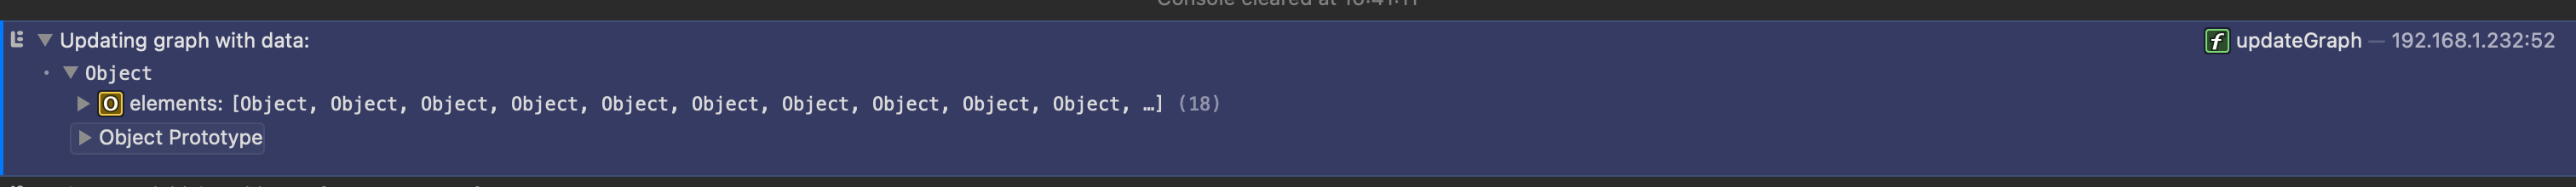
\includegraphics[width=0.8\textwidth]{Prototype/8_Backend/media/V1.png}
    \caption{Data recieved by browser}
\end{figure}
\textbf{Code:}
\inputminted[linenos, tabsize=1, breaklines]{python3}{Prototype/8_Backend/media/CodeV1.py}



\subsection*{V2:}
These next few version aimed to make my backend interact with a local database for storing information (using the database research I had previously completed)
\textbf{Code:}
\inputminted[linenos, tabsize=1, breaklines]{python3}{Prototype/8_Backend/media/CodeV2.py}


\subsection*{V3:}
This minor version simply added a function to fill my database with some demo data (based on my EP docuemntation:)
\textbf{Code:}
\inputminted[linenos, tabsize=1, breaklines]{python3}{Prototype/8_Backend/media/CodeV3.py}

\subsection*{V4:}
From here all of the updates on the backend are detailed within the frontend features respective prototype.